\section{Matrix multiplication}

Multiplying matrices of a large size is often part of heavy scientific calculations and therefore an important building block in every mathematics library. Unfortunately, with an increasing size of the matrices the computation of the product becomes desperately slow due to an asymptotic runtime complexity of $\mathcal{O}(n^3)$ for a naive attempt. Therefore, several improvements have been tried to speed up the calculation like Strassen's algorithm achieving a runtime complexity of $\mathcal{O}(n^{\log_2 7}) = \mathcal{O}(n^{2.807})$ \ref{} which is faster than the naive version but still does not compute results within a satisfying time.
Nonetheless, modern computing systems can take advantage of one important aspect of the matrix multiplication which is it's embarrassing parallel nature. Each element of the output matrix can be computed completely independent. This potential may not only be used by today's CPU's vector extensions like SSE \footnote{Streaming SIMD Extensions, a vector instruction set extension by Intel supporting 128 bit wide registers to process 4 single precision floats in parallel.} or AVX \footnote{Advanced Vector Extensions, Intel's latest vector instruction set extension featuring 256 bit wide registers to process 8 single precision floats in parallel.}. Especially a GPU can make excellent use of the large number of independent pieces of work to perfectly utilize its hundreds or thousands of cores.

\begin{figure}
\centering
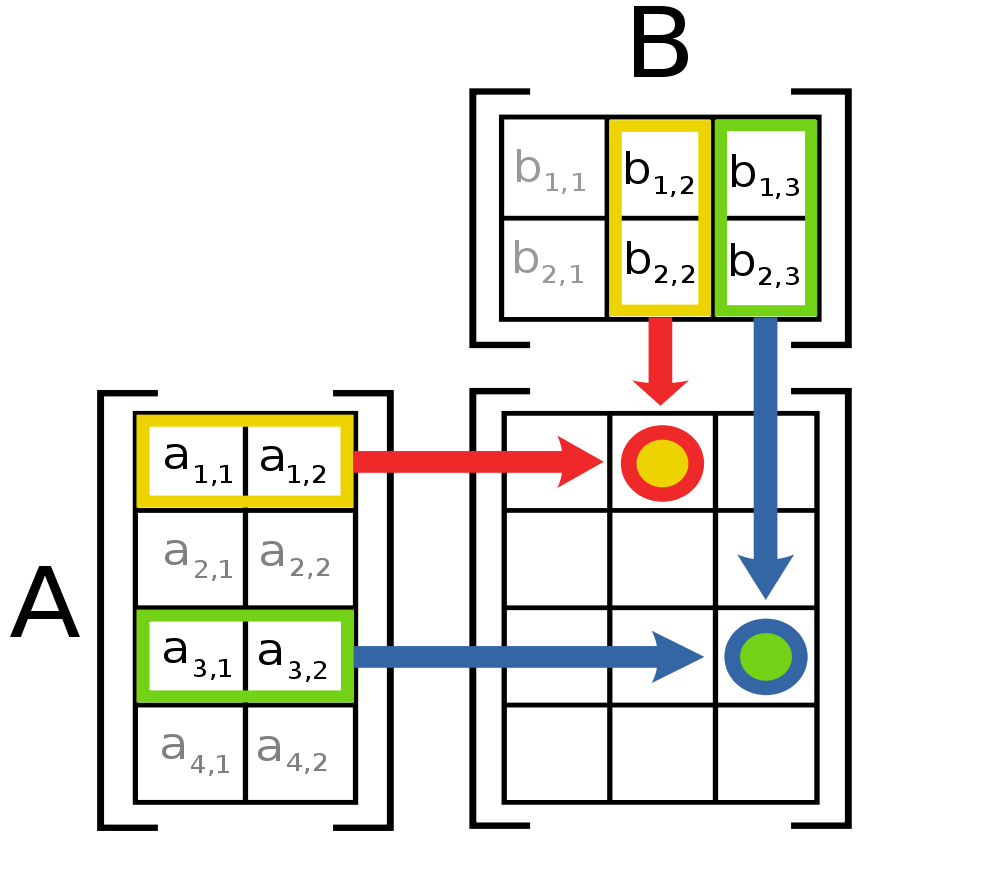
\includegraphics[width=0.5\linewidth]{matrix_mul}
\caption{Principle of the matrix multiplication \cite{wiki_matrix_mul}.}
\label{fig:matrix_mul}
\end{figure}

This chapter will take a look at different implementations of the matrix multiplication for both, the CPU and the GPU. For simplicity, square matrices are used and stored as one dimensional arrays in row major order.

\subsection{CPU Implementation}

Although several optimized implementations exist we will first have a detailed look at a simple naive implementation as given in listing \ref{lst:matrix_cpu}.

\lstset{basicstyle=\ttfamily{}\scriptsize{}}
\lstinputlisting[language=C++, caption=A simple C++ implementation of a square matrix multiplication for the CPU., label=lst:matrix_cpu, firstline=15, lastline=26]{code/matrix/main.cpp}
\lstset{basicstyle=\ttfamily{}}



\begin{figure}
\centering
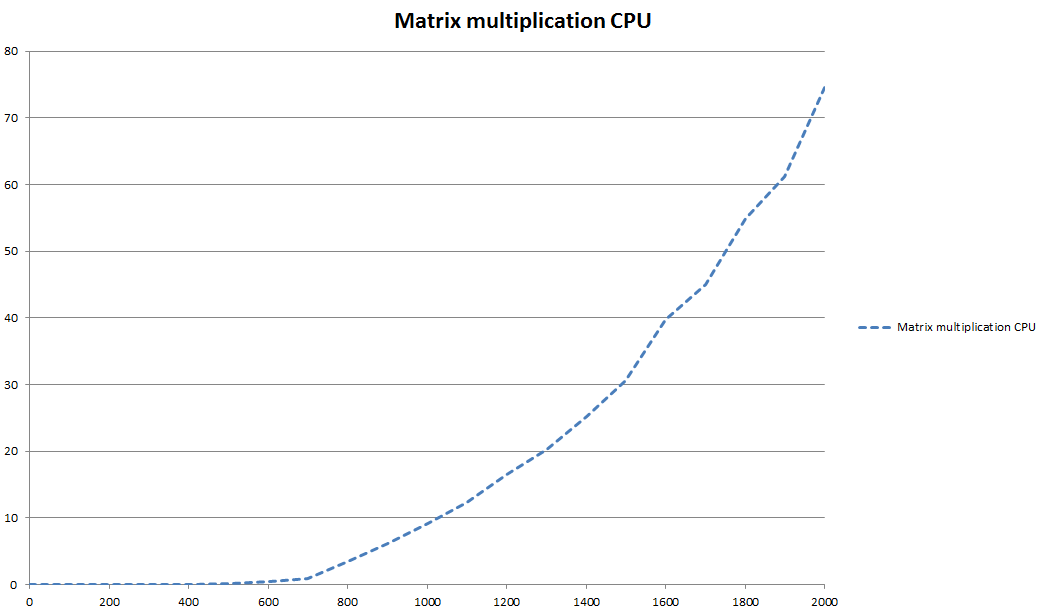
\includegraphics[width=0.9\linewidth]{matrix_cpu}
\caption{Benchmark of the CPU implementation of a square matrix multiplication in listing \ref{lst:matrix_cpu}.}
\label{chart:matrix_cpu}
\end{figure}

\subsection{Naive GPU implementation}

\lstset{basicstyle=\ttfamily{}\scriptsize{}}
\lstinputlisting[language=C++, caption=Host code for a matrix multiplication implementation using OpenCL., label=lst:matrix_cl_naive, firstline=28, lastline=54]{code/matrix/main.cpp}
\lstset{basicstyle=\ttfamily{}}

\lstset{basicstyle=\ttfamily{}\scriptsize{}}
\lstinputlisting[language=CL, caption=OpenCL Kernel code calculating a single element of the output matrix., label=lst:matrix_cl_naive_kernel]{code/matrix/Mult.cl}
\lstset{basicstyle=\ttfamily{}}

approach (how are the elements distributed in work items/groups)
kernel code with explanation
runtime (diagram)

\subsection{Optimized GPU implementation}
options for performance improvement
multiple elements per work item
caching in local memory (blocks)
texture unit
vector instructions

maybe kernel code with explanation

advantages/disadvantages

runtime (diagram)
comparison with CPU and naive GPU implementation

\subsection{Existing implementations}
clAmdBlas
cuBlas
Intel Math Kernel Library (MKL)
AMD COre Math Library (ACML)
(NVIDIA OpenCL Samples)

\subsection{Conclusion}
Which implementation is when better?
commmon diagram
Which problem size?
Which hardware?